\documentclass[12pt]{article}
\usepackage[english]{babel}
\usepackage[utf8x]{inputenc}
\usepackage{amsmath}
\usepackage{tikz}
\usetikzlibrary{arrows,automata}
\begin{document}

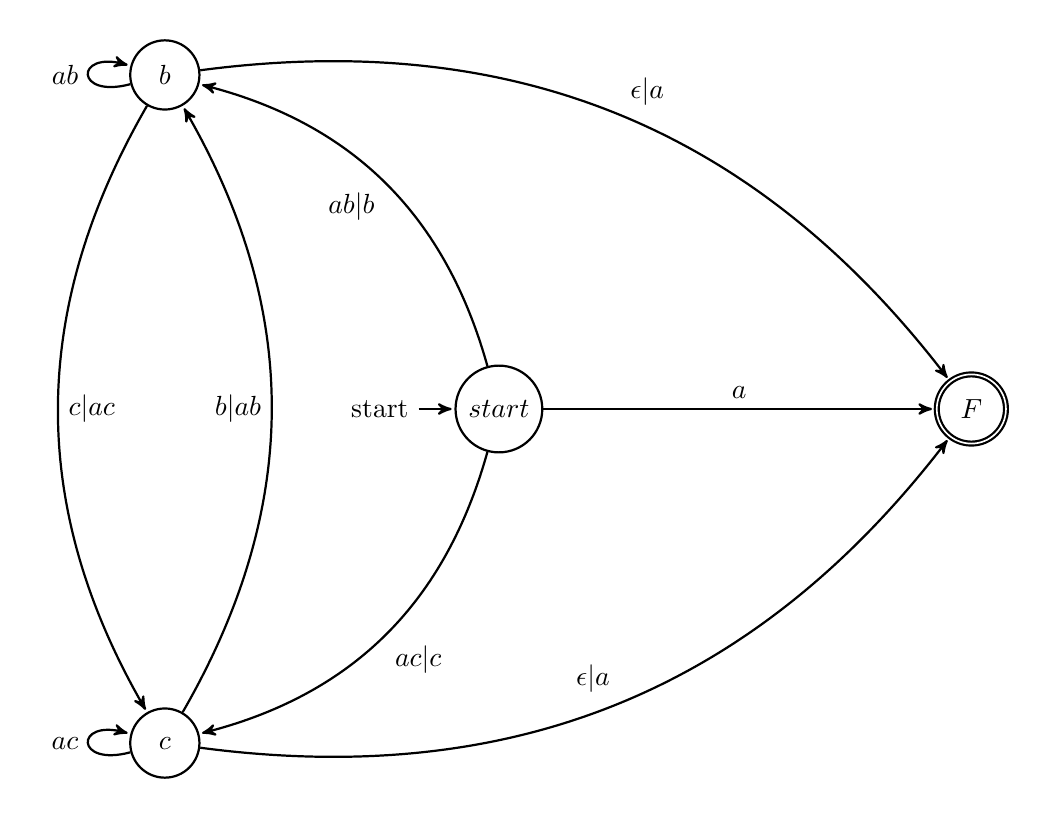
\begin{tikzpicture}[->,>=stealth',shorten >=1pt,auto,node distance=6cm,
    thick,base node/.style={circle,draw,minimum size=8pt}, real node/.style={double,circle,draw,minimum size=17pt}]

  \node[state,initial] (start) {$start$};
  \node[state] (b) [above left of=start] {$b$};
  \node[state] (c) [below left of=start] {$c$};
  \node[state,accepting] (F) [right of=start] {$F$};
  
  \path 
        (start) edge node {$a$} (F)
        (start) edge   [bend right]           node {$ab|b$} (b)
        (start) edge    [bend left]          node {$ac|c$} (c)
        (b)
         edge    [bend right]           node {$c|ac$} (c)
         edge [bend left] node {$\epsilon|a$} (F)
         edge [loop left] node {$ab$} ( )
        (c)
         edge     [bend right]         node {$b|ab$} (b)
         edge  [bend right] node {$\epsilon|a$} (F)
         edge [loop left] node {$ac$} ( )
         ;

\end{tikzpicture}
\end{document}